% Created by tikzDevice version 0.12.6 on 2024-10-09 11:42:55
% !TEX encoding = UTF-8 Unicode
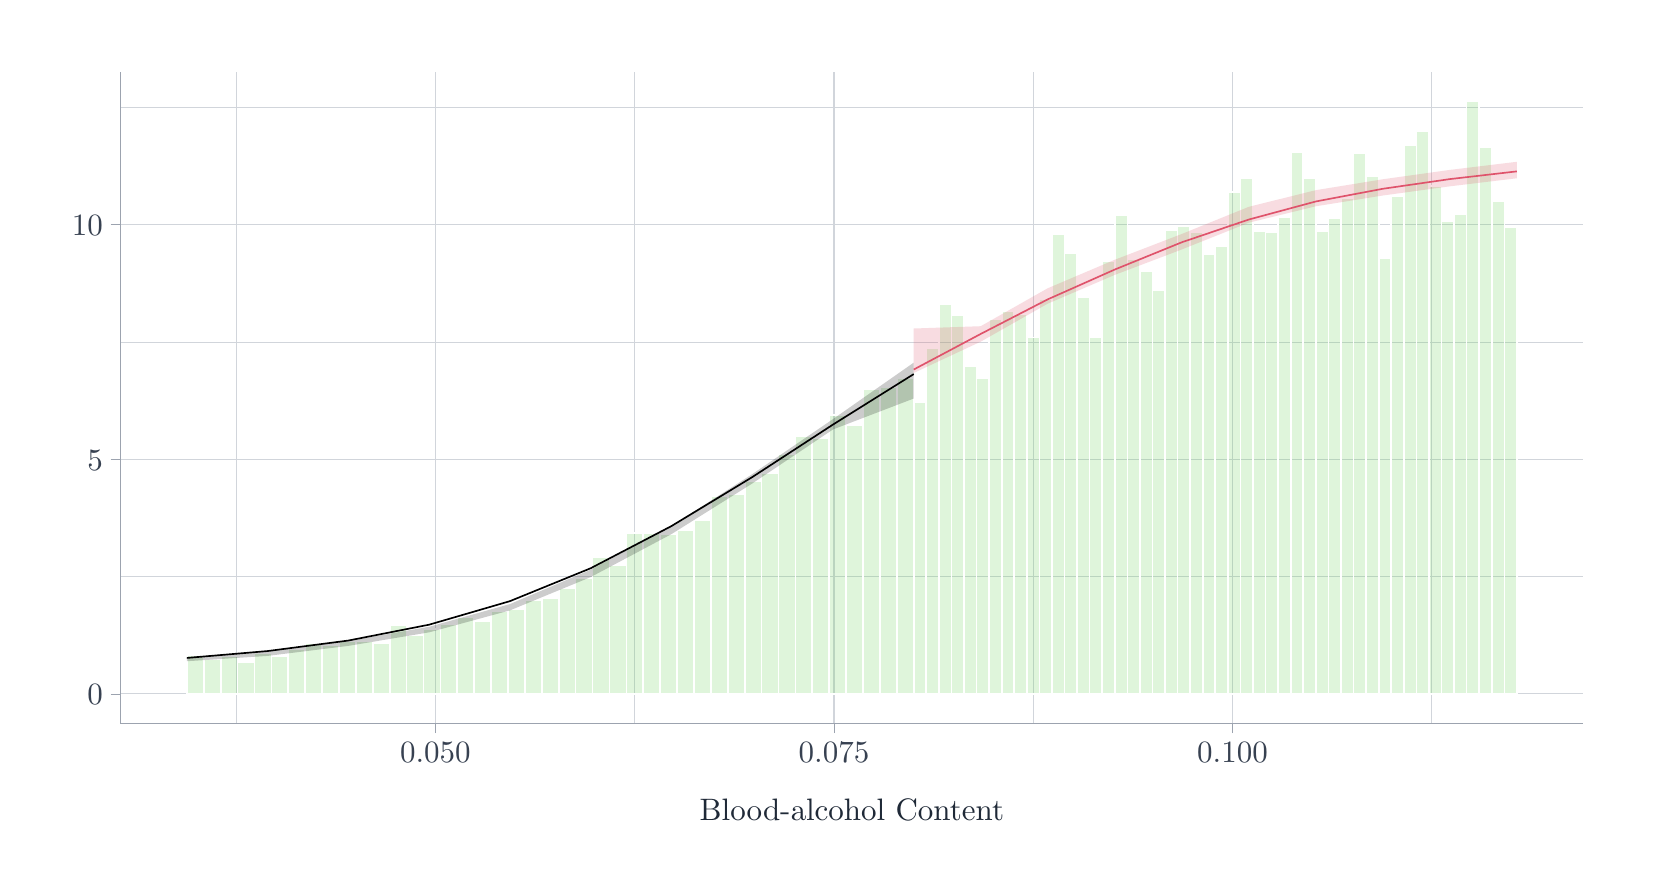
\begin{tikzpicture}[x=1pt,y=1pt]
\definecolor{fillColor}{RGB}{255,255,255}
\path[use as bounding box,fill=fillColor] (0,0) rectangle (578.16,303.53);
\begin{scope}
\path[clip] (  0.00,  0.00) rectangle (578.16,303.53);
\definecolor{drawColor}{RGB}{255,255,255}

\path[draw=drawColor,line width= 0.7pt,line join=round,line cap=round,fill=fillColor] (  0.00,  0.00) rectangle (578.16,303.53);
\end{scope}
\begin{scope}
\path[clip] ( 33.50, 52.08) rectangle (562.16,287.53);
\definecolor{drawColor}{RGB}{255,255,255}
\definecolor{fillColor}{RGB}{255,255,255}

\path[draw=drawColor,line width= 0.7pt,line join=round,line cap=round,fill=fillColor] ( 33.50, 52.08) rectangle (562.16,287.53);
\definecolor{drawColor}{RGB}{209,213,219}

\path[draw=drawColor,line width= 0.4pt,line join=round] ( 33.50,105.15) --
	(562.16,105.15);

\path[draw=drawColor,line width= 0.4pt,line join=round] ( 33.50,189.89) --
	(562.16,189.89);

\path[draw=drawColor,line width= 0.4pt,line join=round] ( 33.50,274.63) --
	(562.16,274.63);

\path[draw=drawColor,line width= 0.4pt,line join=round] ( 75.33, 52.08) --
	( 75.33,287.53);

\path[draw=drawColor,line width= 0.4pt,line join=round] (219.35, 52.08) --
	(219.35,287.53);

\path[draw=drawColor,line width= 0.4pt,line join=round] (363.37, 52.08) --
	(363.37,287.53);

\path[draw=drawColor,line width= 0.4pt,line join=round] (507.39, 52.08) --
	(507.39,287.53);

\path[draw=drawColor,line width= 0.4pt,line join=round] ( 33.50, 62.78) --
	(562.16, 62.78);

\path[draw=drawColor,line width= 0.4pt,line join=round] ( 33.50,147.52) --
	(562.16,147.52);

\path[draw=drawColor,line width= 0.4pt,line join=round] ( 33.50,232.26) --
	(562.16,232.26);

\path[draw=drawColor,line width= 0.4pt,line join=round] (147.34, 52.08) --
	(147.34,287.53);

\path[draw=drawColor,line width= 0.4pt,line join=round] (291.36, 52.08) --
	(291.36,287.53);

\path[draw=drawColor,line width= 0.4pt,line join=round] (435.38, 52.08) --
	(435.38,287.53);
\definecolor{drawColor}{RGB}{255,255,255}
\definecolor{fillColor}{RGB}{97,208,79}

\path[draw=drawColor,line width= 0.6pt,fill=fillColor,fill opacity=0.20] ( 57.53, 62.78) rectangle ( 63.64, 76.72);

\path[draw=drawColor,line width= 0.6pt,fill=fillColor,fill opacity=0.20] ( 63.64, 62.78) rectangle ( 69.74, 75.47);

\path[draw=drawColor,line width= 0.6pt,fill=fillColor,fill opacity=0.20] ( 69.74, 62.78) rectangle ( 75.85, 76.60);

\path[draw=drawColor,line width= 0.6pt,fill=fillColor,fill opacity=0.20] ( 75.85, 62.78) rectangle ( 81.96, 74.22);

\path[draw=drawColor,line width= 0.6pt,fill=fillColor,fill opacity=0.20] ( 81.96, 62.78) rectangle ( 88.07, 77.39);

\path[draw=drawColor,line width= 0.6pt,fill=fillColor,fill opacity=0.20] ( 88.07, 62.78) rectangle ( 94.17, 76.26);

\path[draw=drawColor,line width= 0.6pt,fill=fillColor,fill opacity=0.20] ( 94.17, 62.78) rectangle (100.28, 79.09);

\path[draw=drawColor,line width= 0.6pt,fill=fillColor,fill opacity=0.20] (100.28, 62.78) rectangle (106.39, 81.02);

\path[draw=drawColor,line width= 0.6pt,fill=fillColor,fill opacity=0.20] (106.39, 62.78) rectangle (112.50, 80.34);

\path[draw=drawColor,line width= 0.6pt,fill=fillColor,fill opacity=0.20] (112.50, 62.78) rectangle (118.61, 81.70);

\path[draw=drawColor,line width= 0.6pt,fill=fillColor,fill opacity=0.20] (118.61, 62.78) rectangle (124.71, 81.70);

\path[draw=drawColor,line width= 0.6pt,fill=fillColor,fill opacity=0.20] (124.71, 62.78) rectangle (130.82, 81.25);

\path[draw=drawColor,line width= 0.6pt,fill=fillColor,fill opacity=0.20] (130.82, 62.78) rectangle (136.93, 87.70);

\path[draw=drawColor,line width= 0.6pt,fill=fillColor,fill opacity=0.20] (136.93, 62.78) rectangle (143.04, 84.19);

\path[draw=drawColor,line width= 0.6pt,fill=fillColor,fill opacity=0.20] (143.04, 62.78) rectangle (149.15, 86.23);

\path[draw=drawColor,line width= 0.6pt,fill=fillColor,fill opacity=0.20] (149.15, 62.78) rectangle (155.25, 87.82);

\path[draw=drawColor,line width= 0.6pt,fill=fillColor,fill opacity=0.20] (155.25, 62.78) rectangle (161.36, 90.42);

\path[draw=drawColor,line width= 0.6pt,fill=fillColor,fill opacity=0.20] (161.36, 62.78) rectangle (167.47, 88.95);

\path[draw=drawColor,line width= 0.6pt,fill=fillColor,fill opacity=0.20] (167.47, 62.78) rectangle (173.58, 92.57);

\path[draw=drawColor,line width= 0.6pt,fill=fillColor,fill opacity=0.20] (173.58, 62.78) rectangle (179.68, 93.25);

\path[draw=drawColor,line width= 0.6pt,fill=fillColor,fill opacity=0.20] (179.68, 62.78) rectangle (185.79, 96.76);

\path[draw=drawColor,line width= 0.6pt,fill=fillColor,fill opacity=0.20] (185.79, 62.78) rectangle (191.90, 97.56);

\path[draw=drawColor,line width= 0.6pt,fill=fillColor,fill opacity=0.20] (191.90, 62.78) rectangle (198.01,101.07);

\path[draw=drawColor,line width= 0.6pt,fill=fillColor,fill opacity=0.20] (198.01, 62.78) rectangle (204.12,104.58);

\path[draw=drawColor,line width= 0.6pt,fill=fillColor,fill opacity=0.20] (204.12, 62.78) rectangle (210.22,112.28);

\path[draw=drawColor,line width= 0.6pt,fill=fillColor,fill opacity=0.20] (210.22, 62.78) rectangle (216.33,109.34);

\path[draw=drawColor,line width= 0.6pt,fill=fillColor,fill opacity=0.20] (216.33, 62.78) rectangle (222.44,120.89);

\path[draw=drawColor,line width= 0.6pt,fill=fillColor,fill opacity=0.20] (222.44, 62.78) rectangle (228.55,120.77);

\path[draw=drawColor,line width= 0.6pt,fill=fillColor,fill opacity=0.20] (228.55, 62.78) rectangle (234.66,120.55);

\path[draw=drawColor,line width= 0.6pt,fill=fillColor,fill opacity=0.20] (234.66, 62.78) rectangle (240.76,122.13);

\path[draw=drawColor,line width= 0.6pt,fill=fillColor,fill opacity=0.20] (240.76, 62.78) rectangle (246.87,125.42);

\path[draw=drawColor,line width= 0.6pt,fill=fillColor,fill opacity=0.20] (246.87, 62.78) rectangle (252.98,134.25);

\path[draw=drawColor,line width= 0.6pt,fill=fillColor,fill opacity=0.20] (252.98, 62.78) rectangle (259.09,134.82);

\path[draw=drawColor,line width= 0.6pt,fill=fillColor,fill opacity=0.20] (259.09, 62.78) rectangle (265.20,139.69);

\path[draw=drawColor,line width= 0.6pt,fill=fillColor,fill opacity=0.20] (265.20, 62.78) rectangle (271.30,142.63);

\path[draw=drawColor,line width= 0.6pt,fill=fillColor,fill opacity=0.20] (271.30, 62.78) rectangle (277.41,149.32);

\path[draw=drawColor,line width= 0.6pt,fill=fillColor,fill opacity=0.20] (277.41, 62.78) rectangle (283.52,156.00);

\path[draw=drawColor,line width= 0.6pt,fill=fillColor,fill opacity=0.20] (283.52, 62.78) rectangle (289.63,155.32);

\path[draw=drawColor,line width= 0.6pt,fill=fillColor,fill opacity=0.20] (289.63, 62.78) rectangle (295.73,163.47);

\path[draw=drawColor,line width= 0.6pt,fill=fillColor,fill opacity=0.20] (295.73, 62.78) rectangle (301.84,159.74);

\path[draw=drawColor,line width= 0.6pt,fill=fillColor,fill opacity=0.20] (301.84, 62.78) rectangle (307.95,172.76);

\path[draw=drawColor,line width= 0.6pt,fill=fillColor,fill opacity=0.20] (307.95, 62.78) rectangle (314.06,173.78);

\path[draw=drawColor,line width= 0.6pt,fill=fillColor,fill opacity=0.20] (314.06, 62.78) rectangle (320.17,176.73);

\path[draw=drawColor,line width= 0.6pt,fill=fillColor,fill opacity=0.20] (320.17, 62.78) rectangle (324.71,168.21);

\path[draw=drawColor,line width= 0.6pt,fill=fillColor,fill opacity=0.20] (324.71, 62.78) rectangle (329.25,187.71);

\path[draw=drawColor,line width= 0.6pt,fill=fillColor,fill opacity=0.20] (329.25, 62.78) rectangle (333.79,203.71);

\path[draw=drawColor,line width= 0.6pt,fill=fillColor,fill opacity=0.20] (333.79, 62.78) rectangle (338.33,199.74);

\path[draw=drawColor,line width= 0.6pt,fill=fillColor,fill opacity=0.20] (338.33, 62.78) rectangle (342.87,181.31);

\path[draw=drawColor,line width= 0.6pt,fill=fillColor,fill opacity=0.20] (342.87, 62.78) rectangle (347.41,177.04);

\path[draw=drawColor,line width= 0.6pt,fill=fillColor,fill opacity=0.20] (347.41, 62.78) rectangle (351.95,198.07);

\path[draw=drawColor,line width= 0.6pt,fill=fillColor,fill opacity=0.20] (351.95, 62.78) rectangle (356.49,200.96);

\path[draw=drawColor,line width= 0.6pt,fill=fillColor,fill opacity=0.20] (356.49, 62.78) rectangle (361.03,199.90);

\path[draw=drawColor,line width= 0.6pt,fill=fillColor,fill opacity=0.20] (361.03, 62.78) rectangle (365.58,191.52);

\path[draw=drawColor,line width= 0.6pt,fill=fillColor,fill opacity=0.20] (365.58, 62.78) rectangle (370.12,205.53);

\path[draw=drawColor,line width= 0.6pt,fill=fillColor,fill opacity=0.20] (370.12, 62.78) rectangle (374.66,228.99);

\path[draw=drawColor,line width= 0.6pt,fill=fillColor,fill opacity=0.20] (374.66, 62.78) rectangle (379.20,222.14);

\path[draw=drawColor,line width= 0.6pt,fill=fillColor,fill opacity=0.20] (379.20, 62.78) rectangle (383.74,206.14);

\path[draw=drawColor,line width= 0.6pt,fill=fillColor,fill opacity=0.20] (383.74, 62.78) rectangle (388.28,191.67);

\path[draw=drawColor,line width= 0.6pt,fill=fillColor,fill opacity=0.20] (388.28, 62.78) rectangle (392.82,219.09);

\path[draw=drawColor,line width= 0.6pt,fill=fillColor,fill opacity=0.20] (392.82, 62.78) rectangle (397.36,235.85);

\path[draw=drawColor,line width= 0.6pt,fill=fillColor,fill opacity=0.20] (397.36, 62.78) rectangle (401.90,219.70);

\path[draw=drawColor,line width= 0.6pt,fill=fillColor,fill opacity=0.20] (401.90, 62.78) rectangle (406.44,215.59);

\path[draw=drawColor,line width= 0.6pt,fill=fillColor,fill opacity=0.20] (406.44, 62.78) rectangle (410.98,208.58);

\path[draw=drawColor,line width= 0.6pt,fill=fillColor,fill opacity=0.20] (410.98, 62.78) rectangle (415.53,230.52);

\path[draw=drawColor,line width= 0.6pt,fill=fillColor,fill opacity=0.20] (415.53, 62.78) rectangle (420.07,231.89);

\path[draw=drawColor,line width= 0.6pt,fill=fillColor,fill opacity=0.20] (420.07, 62.78) rectangle (424.61,229.60);

\path[draw=drawColor,line width= 0.6pt,fill=fillColor,fill opacity=0.20] (424.61, 62.78) rectangle (429.15,221.83);

\path[draw=drawColor,line width= 0.6pt,fill=fillColor,fill opacity=0.20] (429.15, 62.78) rectangle (433.69,224.73);

\path[draw=drawColor,line width= 0.6pt,fill=fillColor,fill opacity=0.20] (433.69, 62.78) rectangle (438.23,244.23);

\path[draw=drawColor,line width= 0.6pt,fill=fillColor,fill opacity=0.20] (438.23, 62.78) rectangle (442.77,249.26);

\path[draw=drawColor,line width= 0.6pt,fill=fillColor,fill opacity=0.20] (442.77, 62.78) rectangle (447.31,230.06);

\path[draw=drawColor,line width= 0.6pt,fill=fillColor,fill opacity=0.20] (447.31, 62.78) rectangle (451.85,229.76);

\path[draw=drawColor,line width= 0.6pt,fill=fillColor,fill opacity=0.20] (451.85, 62.78) rectangle (456.39,234.94);

\path[draw=drawColor,line width= 0.6pt,fill=fillColor,fill opacity=0.20] (456.39, 62.78) rectangle (460.93,258.40);

\path[draw=drawColor,line width= 0.6pt,fill=fillColor,fill opacity=0.20] (460.93, 62.78) rectangle (465.48,249.10);

\path[draw=drawColor,line width= 0.6pt,fill=fillColor,fill opacity=0.20] (465.48, 62.78) rectangle (470.02,229.91);

\path[draw=drawColor,line width= 0.6pt,fill=fillColor,fill opacity=0.20] (470.02, 62.78) rectangle (474.56,234.63);

\path[draw=drawColor,line width= 0.6pt,fill=fillColor,fill opacity=0.20] (474.56, 62.78) rectangle (479.10,241.94);

\path[draw=drawColor,line width= 0.6pt,fill=fillColor,fill opacity=0.20] (479.10, 62.78) rectangle (483.64,258.25);

\path[draw=drawColor,line width= 0.6pt,fill=fillColor,fill opacity=0.20] (483.64, 62.78) rectangle (488.18,249.71);

\path[draw=drawColor,line width= 0.6pt,fill=fillColor,fill opacity=0.20] (488.18, 62.78) rectangle (492.72,220.31);

\path[draw=drawColor,line width= 0.6pt,fill=fillColor,fill opacity=0.20] (492.72, 62.78) rectangle (497.26,242.55);

\path[draw=drawColor,line width= 0.6pt,fill=fillColor,fill opacity=0.20] (497.26, 62.78) rectangle (501.80,260.99);

\path[draw=drawColor,line width= 0.6pt,fill=fillColor,fill opacity=0.20] (501.80, 62.78) rectangle (506.34,266.01);

\path[draw=drawColor,line width= 0.6pt,fill=fillColor,fill opacity=0.20] (506.34, 62.78) rectangle (510.88,246.21);

\path[draw=drawColor,line width= 0.6pt,fill=fillColor,fill opacity=0.20] (510.88, 62.78) rectangle (515.43,233.57);

\path[draw=drawColor,line width= 0.6pt,fill=fillColor,fill opacity=0.20] (515.43, 62.78) rectangle (519.97,236.15);

\path[draw=drawColor,line width= 0.6pt,fill=fillColor,fill opacity=0.20] (519.97, 62.78) rectangle (524.51,276.83);

\path[draw=drawColor,line width= 0.6pt,fill=fillColor,fill opacity=0.20] (524.51, 62.78) rectangle (529.05,260.23);

\path[draw=drawColor,line width= 0.6pt,fill=fillColor,fill opacity=0.20] (529.05, 62.78) rectangle (533.59,240.73);

\path[draw=drawColor,line width= 0.6pt,fill=fillColor,fill opacity=0.20] (533.59, 62.78) rectangle (538.13,231.58);
\definecolor{fillColor}{RGB}{0,0,0}

\path[fill=fillColor,fill opacity=0.20] ( 57.53, 76.06) --
	( 86.71, 78.09) --
	(115.89, 81.91) --
	(145.07, 87.04) --
	(174.26, 95.25) --
	(203.44,107.65) --
	(232.62,123.47) --
	(261.80,142.18) --
	(290.98,162.07) --
	(320.17,182.49) --
	(320.17,169.52) --
	(290.98,158.34) --
	(261.80,138.80) --
	(232.62,120.52) --
	(203.44,104.99) --
	(174.26, 92.96) --
	(145.07, 85.03) --
	(115.89, 80.14) --
	( 86.71, 76.52) --
	( 57.53, 74.59) --
	cycle;

\path[] ( 57.53, 76.06) --
	( 86.71, 78.09) --
	(115.89, 81.91) --
	(145.07, 87.04) --
	(174.26, 95.25) --
	(203.44,107.65) --
	(232.62,123.47) --
	(261.80,142.18) --
	(290.98,162.07) --
	(320.17,182.49);

\path[] (320.17,169.52) --
	(290.98,158.34) --
	(261.80,138.80) --
	(232.62,120.52) --
	(203.44,104.99) --
	(174.26, 92.96) --
	(145.07, 85.03) --
	(115.89, 80.14) --
	( 86.71, 76.52) --
	( 57.53, 74.59);
\definecolor{drawColor}{RGB}{0,0,0}

\path[draw=drawColor,line width= 0.6pt,line join=round] ( 57.53, 75.78) --
	( 86.71, 78.27) --
	(115.89, 82.07) --
	(145.07, 87.80) --
	(174.26, 96.30) --
	(203.44,108.19) --
	(232.62,123.43) --
	(261.80,141.11) --
	(290.98,160.10) --
	(320.17,178.35);
\definecolor{fillColor}{RGB}{223,83,107}

\path[fill=fillColor,fill opacity=0.20] (320.17,194.82) --
	(344.38,195.65) --
	(368.60,209.37) --
	(392.82,219.66) --
	(417.04,228.98) --
	(441.26,238.80) --
	(465.48,244.81) --
	(489.69,248.75) --
	(513.91,252.13) --
	(538.13,255.06) --
	(538.13,249.11) --
	(513.91,246.20) --
	(489.69,242.88) --
	(465.48,238.99) --
	(441.26,233.06) --
	(417.04,223.38) --
	(392.82,214.19) --
	(368.60,203.80) --
	(344.38,190.07) --
	(320.17,178.76) --
	cycle;

\path[] (320.17,194.82) --
	(344.38,195.65) --
	(368.60,209.37) --
	(392.82,219.66) --
	(417.04,228.98) --
	(441.26,238.80) --
	(465.48,244.81) --
	(489.69,248.75) --
	(513.91,252.13) --
	(538.13,255.06);

\path[] (538.13,249.11) --
	(513.91,246.20) --
	(489.69,242.88) --
	(465.48,238.99) --
	(441.26,233.06) --
	(417.04,223.38) --
	(392.82,214.19) --
	(368.60,203.80) --
	(344.38,190.07) --
	(320.17,178.76);
\definecolor{drawColor}{RGB}{223,83,107}

\path[draw=drawColor,line width= 0.6pt,line join=round] (320.17,180.00) --
	(344.38,192.86) --
	(368.60,205.35) --
	(392.82,216.13) --
	(417.04,225.98) --
	(441.26,234.20) --
	(465.48,240.73) --
	(489.69,245.31) --
	(513.91,248.81) --
	(538.13,251.60);
\end{scope}
\begin{scope}
\path[clip] (  0.00,  0.00) rectangle (578.16,303.53);
\definecolor{drawColor}{RGB}{156,163,175}

\path[draw=drawColor,line width= 0.3pt,line join=round] ( 33.50, 52.08) --
	( 33.50,287.53);
\end{scope}
\begin{scope}
\path[clip] (  0.00,  0.00) rectangle (578.16,303.53);
\definecolor{drawColor}{RGB}{55,65,81}

\node[text=drawColor,anchor=base east,inner sep=0pt, outer sep=0pt, scale=  1.12] at ( 27.20, 58.93) {0};

\node[text=drawColor,anchor=base east,inner sep=0pt, outer sep=0pt, scale=  1.12] at ( 27.20,143.67) {5};

\node[text=drawColor,anchor=base east,inner sep=0pt, outer sep=0pt, scale=  1.12] at ( 27.20,228.40) {10};
\end{scope}
\begin{scope}
\path[clip] (  0.00,  0.00) rectangle (578.16,303.53);
\definecolor{drawColor}{RGB}{156,163,175}

\path[draw=drawColor,line width= 0.3pt,line join=round] ( 30.00, 62.78) --
	( 33.50, 62.78);

\path[draw=drawColor,line width= 0.3pt,line join=round] ( 30.00,147.52) --
	( 33.50,147.52);

\path[draw=drawColor,line width= 0.3pt,line join=round] ( 30.00,232.26) --
	( 33.50,232.26);
\end{scope}
\begin{scope}
\path[clip] (  0.00,  0.00) rectangle (578.16,303.53);
\definecolor{drawColor}{RGB}{156,163,175}

\path[draw=drawColor,line width= 0.3pt,line join=round] ( 33.50, 52.08) --
	(562.16, 52.08);
\end{scope}
\begin{scope}
\path[clip] (  0.00,  0.00) rectangle (578.16,303.53);
\definecolor{drawColor}{RGB}{156,163,175}

\path[draw=drawColor,line width= 0.3pt,line join=round] (147.34, 48.58) --
	(147.34, 52.08);

\path[draw=drawColor,line width= 0.3pt,line join=round] (291.36, 48.58) --
	(291.36, 52.08);

\path[draw=drawColor,line width= 0.3pt,line join=round] (435.38, 48.58) --
	(435.38, 52.08);
\end{scope}
\begin{scope}
\path[clip] (  0.00,  0.00) rectangle (578.16,303.53);
\definecolor{drawColor}{RGB}{55,65,81}

\node[text=drawColor,anchor=base,inner sep=0pt, outer sep=0pt, scale=  1.12] at (147.34, 38.07) {0.050};

\node[text=drawColor,anchor=base,inner sep=0pt, outer sep=0pt, scale=  1.12] at (291.36, 38.07) {0.075};

\node[text=drawColor,anchor=base,inner sep=0pt, outer sep=0pt, scale=  1.12] at (435.38, 38.07) {0.100};
\end{scope}
\begin{scope}
\path[clip] (  0.00,  0.00) rectangle (578.16,303.53);
\definecolor{drawColor}{RGB}{31,41,55}

\node[text=drawColor,anchor=base,inner sep=0pt, outer sep=0pt, scale=  1.12] at (297.83, 17.09) {Blood-alcohol Content};
\end{scope}
\end{tikzpicture}
